\documentclass[a4paper,12pt]{article}
\usepackage{amsmath, amssymb, mathrsfs, graphicx, xcolor}
\usepackage[margin=1in]{geometry}
\usepackage{array}

\begin{document}

\begin{center}
    {\Huge \textbf{DAVE3705-1 25V FORMELARK}}
\end{center}


\renewcommand{\arraystretch}{1.8}
\begin{tabular}{ |c|c| }
    \hline
    \textbf{Function} & \textbf{Laplace Transform} \\
    \hline
    $f(t)$ & $F(s) = \int_{0}^{\infty} e^{-st} f(t) dt$ \\
    \hline
    $a f(t) + b g(t)$ & $a F(s) + b G(s)$ \\
    \hline
    $f'(t)$ & $s F(s) - f(0)$ \\
    \hline
    $f''(t)$ & $s^2 F(s) - s f(0) - f'(0)$ \\
    \hline
    $f'''(t)$ & $s^3 F(s) - s^2 f(0) - s f'(0) - f''(0)$ \\
    \hline
    $f^{(n)}(t)$ & $s^n F(s) - \sum_{k=0}^{n-1} s^{n-1-k} f^{(k)}(0)$ \\
    \hline
    $\int_{0}^{t} f(\tau) d\tau$ & $\frac{F(s)}{s}$ \\
    \hline
    $e^{at} f(t)$ & $F(s-a)$ \\
    \hline
    $u(t-a) f(t-a)$ & $e^{-as} F(s)$ \\
    \hline
    $\int_{0}^{t} f(\tau) g(t-\tau) d\tau$ & $F(s) G(s)$ \\
    \hline
    $t f(t)$ & $-F'(s)$ \\
    \hline
    $t^n f(t)$ & $(-1)^n F^{(n)}(s)$ \\
    \hline
    $\frac{f(t)}{t}$ & $\int_{s}^{\infty} F(\sigma) d\sigma$ \\
    \hline
    $f(t+p) = f(p)$ (periodic function) & $\frac{1}{1 - e^{-ps}} \int_{0}^{p} e^{-st} f(t) dt$ \\
    \hline
\end{tabular}




\section*{Laplace Transforms of Common Functions}
\begin{tabular}{ |c|c| }
    \hline
    \textbf{Function} & \textbf{Laplace Transform} \\
    \hline
    $1$ & $\frac{1}{s}$ \\
    \hline
    $t$ & $\frac{1}{s^2}$ \\
    \hline
    $t^n$ & $\frac{n!}{s^{n+1}}$ \\
    \hline
    $t^a$ & $\frac{\Gamma(a+1)}{s^{a+1}}$ \\
    \hline
    $e^{at}$ & $\frac{1}{s-a}$ \\
    \hline
    $t^n e^{at}$ & $\frac{n!}{(s-a)^{n+1}}$ \\
    \hline
    $\cos(kt)$ & $\frac{s}{s^2 + k^2}$ \\
    \hline
    $\sin(kt)$ & $\frac{k}{s^2 + k^2}$ \\
    \hline
    $e^{at} \cos(kt)$ & $\frac{s-a}{(s-a)^2 + k^2}$ \\
    \hline
    $e^{at} \sin(kt)$ & $\frac{k}{(s-a)^2 + k^2}$ \\
    \hline
    $\frac{t}{2k} \sin(kt)$ & $\frac{s}{(s^2 + k^2)^2}$ \\
    \hline
    $u(t-a)$ (step function) & $e^{-as}$ \\
    \hline
\end{tabular}

\section*{Derivatives}
\renewcommand{\arraystretch}{1.8}
\begin{tabular}{ |c|c| }
    \hline
    \textbf{Function} & \textbf{Derivative} \\
    \hline
    $\ln x$ & $\frac{1}{x}$ \\
    \hline
    $a^x$ & $a^x \ln a$ \\
    \hline
    $\sin x$ & $\cos x$ \\
    \hline
    $\cos x$ & $-\sin x$ \\
    \hline
    $x^a$ & $a x^{a-1}$ \\
    \hline
    $(f(x) \cdot g(x))'$ & $f'(x) \cdot g(x) + f(x) \cdot g'(x)$ \\
    \hline
    $f(x) = h(g(x))$ & $h'(g(x)) \cdot g'(x)$ \\
    \hline
\end{tabular}

\newpage
\section*{Partial Fraction Expansion}
\begin{equation*}
    \frac{p x + q}{(x - a)^2} = \frac{A}{x - a} + \frac{B}{(x - a)^2}
\end{equation*}

\begin{equation*}
    \frac{p x^2 + q x + r}{(x - a)^2 (x - b)} = \frac{A}{x - a} + \frac{B}{(x - a)^2} + \frac{C}{x - b}
\end{equation*}

\section*{Trigonometric Functions}
\begin{equation*}
    \cos(\alpha + \beta) = \cos \alpha \cos \beta - \sin \alpha \sin \beta
\end{equation*}

\begin{equation*}
    \sin(\alpha + \beta) = \sin \alpha \cos \beta + \cos \alpha \sin \beta
\end{equation*}

\section*{Partial Fraction Expansion}
\begin{equation*}
    \frac{p x + q}{(x - a)^2} = \frac{A}{x - a} + \frac{B}{(x - a)^2}
\end{equation*}

\begin{equation*}
    \frac{p x^2 + q x + r}{(x - a)^2 (x - b)} = \frac{A}{x - a} + \frac{B}{(x - a)^2} + \frac{C}{x - b}
\end{equation*}

\section*{Trigonometric Functions}
\begin{equation*}
    \cos(\alpha + \beta) = \cos \alpha \cos \beta - \sin \alpha \sin \beta
\end{equation*}

\begin{equation*}
    \sin(\alpha + \beta) = \sin \alpha \cos \beta + \cos \alpha \sin \beta
\end{equation*}
\newpage
\section*{Integrals}
\begin{equation*}
    \int a\,dx = ax + C
\end{equation*}

\begin{equation*}
    \int x^n dx = \frac{x^{n+1}}{n+1} + C
\end{equation*}

\begin{equation*}
    \int \frac{dx}{x} = \ln |x| + C
\end{equation*}

\begin{equation*}
    \int \frac{c}{ax + b} dx = \frac{c}{a} \ln |ax + b| + C
\end{equation*}

\begin{equation*}
    \int e^{ax} dx = \frac{1}{a} e^{ax} + C
\end{equation*}

\begin{equation*}
    \int \sin x\,dx = -\cos x + C
\end{equation*}

\begin{equation*}
    \int \cos x\,dx = \sin x + C
\end{equation*}

\begin{equation*}
    \int \sin^2 x\,dx = \frac{1}{2} \left( x - \frac{\sin 2x}{2} \right) + C
\end{equation*}

\begin{equation*}
    \int \cos^2 x\,dx = \frac{1}{2} \left( x + \frac{\sin 2x}{2} \right) + C
\end{equation*}

\begin{equation*}
    \int x \cos(ax) dx = \frac{\cos(ax)}{a^2} + \frac{x \sin(ax)}{a} + C
\end{equation*}

\begin{equation*}
    \int x \sin(ax) dx = \frac{\sin(ax)}{a^2} - \frac{x \cos(ax)}{a} + C
\end{equation*}

\section*{Fourier Series}
For $f(x + T) = f(x)$, $T = 2L$:
\begin{equation*}
    f(x) = \frac{a_0}{2} + \sum_{n=1}^{\infty} \left( a_n \cos\left(\frac{n \pi}{L} x\right) + b_n \sin\left(\frac{n \pi}{L} x\right) \right)
\end{equation*}

\begin{equation*}
    a_0 = \frac{1}{L} \int_{-L}^{L} f(x)\,dx
\end{equation*}

\begin{equation*}
    a_n = \frac{1}{L} \int_{-L}^{L} f(x) \cos\left(\frac{n \pi}{L} x\right) dx
\end{equation*}

\begin{equation*}
    b_n = \frac{1}{L} \int_{-L}^{L} f(x) \sin\left(\frac{n \pi}{L} x\right) dx
\end{equation*}

\subsection*{If $f(x)$ is Antisymmetric (Odd):}
If $f(-x) = -f(x)$, then:
\begin{center}
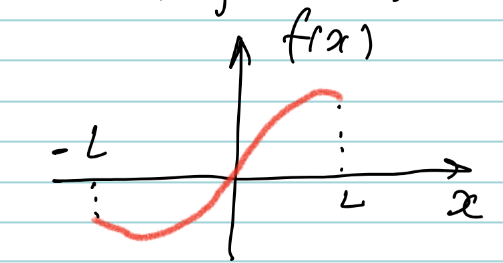
\includegraphics[width=0.2\textwidth]{Bilder/1.png}
\end{center}
\begin{equation*}
    a_0 = a_n = 0 
\end{equation*}

\begin{equation*}
    b_n = \frac{2}{L} \int_{0}^{L} f(x) \sin\left(\frac{n \pi}{L} x\right) dx
\end{equation*}

\subsection*{If $f(x)$ is Symmetric (Even):}
If $f(-x) = f(x)$, then:
\begin{center}
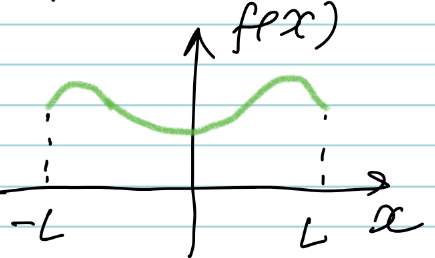
\includegraphics[width=0.2\textwidth]{Bilder/2.png}
\end{center}
\begin{equation*}
    b_n = 0
\end{equation*}

\begin{equation*}
    a_n = \frac{2}{L} \int_{0}^{L} f(x) \cos\left(\frac{n \pi}{L} x\right) dx
\end{equation*}


\section*{Characteristic Equation Method}
The general form of a second-order differential equation:
\begin{equation*}
    a y''(x) + b y'(x) + c y(x) = 0
\end{equation*}

Using the ansatz $y(x) = e^{rx}$, we obtain the characteristic equation:
\begin{equation*}
    a r^2 + b r + c = 0 \Rightarrow r_{1,2} = \frac{-b \pm \sqrt{b^2 - 4ac}}{2a}
\end{equation*}

\subsection*{Distinct Roots: $r_1 \neq r_2$, both real}
\begin{equation*}
    y(x) = C_1 e^{r_1 x} + C_2 e^{r_2 x}
\end{equation*}

\subsection*{Single Root: $r_1 = r_2 = r$}
\begin{equation*}
    y(x) = C_1 e^{r x} + C_2 x e^{r x}
\end{equation*}

\subsection*{Complex Roots: $r_{1,2} = \alpha \pm i\beta$}
\begin{equation*}
    y(x) = e^{\alpha x} \left( C_1 \cos \beta x + C_2 \sin \beta x \right)
\end{equation*}
\newpage
\section*{Heat Equation}
In one dimension:
\begin{equation*}
    \frac{\partial u}{\partial t} = k \frac{\partial^2 u}{\partial x^2}
\end{equation*}

\subsection*{Boundary Conditions:}
\begin{itemize}
    \item $u(0,t) = 0$, $u(L,t) = 0$ (Zero temperature at the ends of the rod)
    \item $u_x(0,t) = 0$, $u_x(L,t) = 0$ (Insulated ends)
\end{itemize}

\subsection*{Initial Condition:}
\begin{equation*}
    u(x,0) = f(x)
\end{equation*}

\section*{Method to Solve: Separation of Variables}
Assume:
\begin{equation*}
    u(x,t) = X(x) T(t)
\end{equation*}

Substituting into the equation:
\begin{equation*}
    \frac{\dot{T}(t)}{kT(t)} = \frac{X''(x)}{X(x)} = \text{constant} = -\lambda
\end{equation*}


\section*{Solution for Zero-Temperature End Boundary Condition}
\begin{equation*}
    u(x,t) = \sum_{n=1}^{\infty} b_n e^{-\frac{n^2 \pi^2}{L^2} kt} \sin\left(\frac{n \pi}{L} x\right)
\end{equation*}

where
\begin{equation*}
    b_n = \frac{2}{L} \int_{0}^{L} f(x) \sin\left(\frac{n \pi}{L} x\right) dx
\end{equation*}

\section*{Solution for Insulated Ends}
\begin{equation*}
    u(x,t) = \frac{a_0}{2} + \sum_{n=1}^{\infty} a_n \exp\left(-\frac{n^2 \pi^2}{L^2} k t\right) \cos\left(\frac{n \pi}{L} x\right)
\end{equation*}

where
\begin{equation*}
    a_n = \frac{2}{L} \int_{0}^{L} f(x) \cos\left(\frac{n \pi}{L} x\right) dx
\end{equation*}


\section*{Wave Equation}
In one dimension:
\begin{equation*}
    \frac{\partial^2 y}{\partial t^2} = a^2 \frac{\partial^2 y}{\partial x^2}
\end{equation*}

\[
    \left\{
    \begin{array}{ll}
        y(0,t) = 0 \\
        y(L,t) = 0
    \end{array}
    \right.
\]


\[
    \left\{
    \begin{array}{ll}
        y(x,0) = f(x) & \text{Initial displacement} \\
        y_t(x,0) = g(x) & \text{Initial velocity}
    \end{array}
    \right.
\]

\section*{Method to Solve: Separation of Variables}
Assume:
\begin{equation*}
    u(x,t) = X(x) T(t)
\end{equation*}




\end{document}
